\section{Design Space}
\label{sec:dspace}

In this section we highlight the size and complexity of the design space of
programmable storage, showing how the ad-hoc approach used in Malacology is
limited by increases in software design and maintenance of co-designed
interfaces. Note that while there are many interfaces in Malacology, we focus
on the \emph{Data I/O} interface for our examples. We report on our experience
building multiple functionally equivalent implementations of the CORFU protocol
in Ceph, and demonstrate that static selection of optimization strategies and
tuning decisions can lead to performance portability challenges.

\subsection{System Tunables and Hardware}

A recent version of Ceph from May 2016 had 994 tunable parameters, controlling
all aspects of the system such as the object storage server (195), low-level
components such as XFS and BlueStore (95), and sub-systems such as RocksDB and
journaling (29). Previous investigations exploring the application of
auto-tuning techniques to systems exhibiting a large space of parameters was
met with limited success~\cite{behzad:sc2013-autotuning}. And challenges
associated with this approach are exacerbated in the context of
application-specific modifications and dynamically changing workloads which
only serve to increase the state space size.

{\bf Hardware.} Ceph is intended to run on a wide variety of commodity,
high-end, and low-end hardware, including newer high-performance non-volatile
storage devices. Each hardware configuration encompasses specific sets of
performance characteristics and tunables (e.g. I/O scheduler selection, and
policies such as timeouts). In our experiments, we tested a variety of
hardware and discovered a wide range of behaviors and performance profiles.
While we generally observe the expected improvements on faster devices, choosing the
best implementation strategy is highly dependent on hardware. This will
continue to be true as storage systems evolve to support new technologies such as
persistent memories and RDMA networks that may require entirely new storage
interfaces for applications to fully exploit the performance of hardware.

\textbf{Takeaway:} Evolving hardware and system tunables presents a challenge
in optimizing systems, even in static cases with fixed workloads. Programmable
storage approaches that introduce application-specific interfaces are
sensitive to changes in workloads and the cost models of
low-level interfaces that are subject to change. This greatly increases the design
space and set of concerns that must be addressed by programmers.

\subsection{Software}
\label{software}

The primary source of complexity in large storage systems is, unsurprisingly,
the vast amount of software written to handle challenges like fault-tolerance
and consistency in distributed heterogeneous environments. We have found that
even routine upgrades can cause performance regressions which manifest as obstacles 
for adopters of a programmable storage approach to development. We use the
CORFU shared-log protocol as a motivating example.

{\bf Shared-log.} In our implementation of CORFU on Ceph~\cite{zlog} the shared-log is striped
across a set of objects in Ceph to provide parallel I/O bandwidth. Each object
implements the custom storage interface that exposes a 64-bit write-once address
space, required by the CORFU protocol.  While this interface can be
built directly into flash devices~\cite{wei:systor13}, we constructed four
different versions in software as native RADOS interfaces in Ceph. Each of our
implementations differs with respect to which internal interfaces are used
(e.g. RocksDB, and/or a bytestream) and how data is striped and partitioned in the system.

Figure~\ref{fig:phy-design} shows the append throughput of four such
implementations running on two versions of Ceph from 2014 and 2016 using the same hardware, in which
the performance in general is significantly better in the newer version of
Ceph. However, if we consider other costs such as software maintenance these results
reveal another trade-off. The top two best implementations running on
the 2014 version of Ceph perform with nearly identical throughput, but
have different implementation complexities. When we consider the performance
of the same implementations on the newer version of Ceph a challenge presents
itself: developers face a reasonable choice between a simpler implementation in the
2014 version of Ceph with little performance difference, and a storage
interface which will perform significantly worse in the 2016 version of Ceph,
requiring a significant overhaul of low-level interface implementations. We
believe that these trade-offs will continue to present themselves as new
hardware is supported and internal storage interfaces evolve.

\begin{figure}
    \centering
    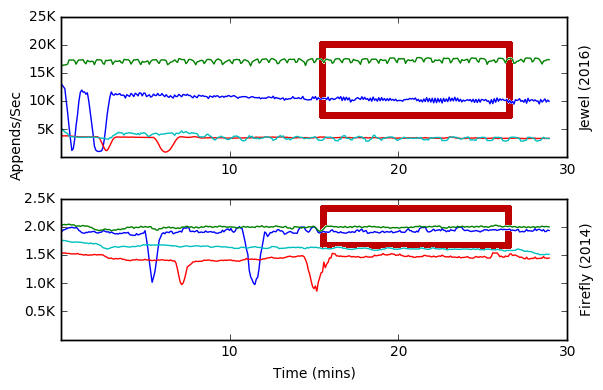
\includegraphics[width=1.0\linewidth]{jewel_v_firefly_pd.png}
    %\caption{Relative performance differences can be drastic after a software
    %upgrade of the underlying storage system.}
    \caption{Performance of four shared-log implementations on two different
    versions Ceph.}
    \label{fig:phy-design}
\end{figure}

{\bf Group commit.} In addition to the broad challenge of design and
implementation, tuning application-specific interfaces for a static
implementation can be challenging.  Group commit is a technique used in
database query execution that combines multiple transactions in order to
amortize over fixed per-transaction costs~\cite{gray}. We implemented two
batching strategies for shared-log appends. The first approach called
\emph{Basic-Batch} groups multiple requests together, but processes each
sub-request (i.e. log append) independently at the lowest level.
The second approach called \emph{Opt-Batch} examines the requests in a batch
and issues efficient low-level I/O requests (e.g. range queries and
data sieving~\cite{750599}). With a batch size of 1 request both approaches achieve
approximately 14K appends per second with a single storage node. With a batch size of 5 requests
\emph{Basic-Batch} and \emph{Opt-Batch} performance increases by 2.3x and 4.2x,
respectively, and with a batch size of 10 requests the increase is 2.7x and 7.0x, achieving
97K appends per second at the high end.

While this batching technique significantly increases throughput, the story is
more complex. The effectiveness of this technique requires tuning parameters
such as forcing request delays to achieve larger batch sizes, which in turn
have a direct effect on latency. While performance of this technique benefited
from using range queries and data sieving, these interfaces are sensitive to
outliers that generate large I/O requests containing a high percentage of
irrelevant data.  In Figure~\ref{fig:batching-outlier} the \emph{Basic-Batch}
case handles each request in a batch independently and, while the resulting
performance is worse relative to the other techniques, it is not sensitive to
outliers. The \emph{Opt-Batch} implementation achieves high append throughput,
but performance degrades as the magnitude of the outliers in the batch
increases due to wasted I/O. In contrast, an \emph{Outlier-Aware} policy
applies a simple heuristic to identify and handle outliers independently,
resulting in only a slight decrease in performance over the best case.

\textbf{Takeaway:} Choosing the best implementation of a storage interface
depends on the timing of development (e.g. system version); the expertise of
programmers and administrators; tuning parameters and hardware configuration;
and system-level and application-specific workload characteristics. A
direct consequence of such a large design space is that some choices may
quickly become sub-optimal as aspects of the system change.  This forces
developers to revise implementations frequently, increasing the risk of introducing bugs that, in the
best case, affect a single application and, in monolithic designs, may
cause systemic data loss.

We believe a better understanding of application and interface semantics
exposes a frontier of new and better approaches with fewer maintenance
requirements than hard-coded and hand-tuned implementations. An ideal solution
to these challenges is an automated system search of
\emph{implementations}---not simply tuning parameters---based on
programmer-produced specifications of storage interfaces in a process
independent of optimization strategies, and guaranteed to not introduce
correctness bugs. Next we'll discuss a candidate approach using a declarative
language for interface specification.
